\section{RAOES Overview}
\label{sec:overview}
The goal of RAOES is to seamlessly support the collaboration of software architects and programmers in event-driven systems' development.
In the latter, the behavior of active objects is specified by using UML State Machines.
To do it, RAOES defines a mechanism interface embedded inside the active objects, which are defined by object-oriented classes. 
This mechanism acts as a role to communicate the C++ programming language to USM so that the traceability between model and code in the reverse direction of the RTE can be eased.

Specifically, in the code generation process, instead of directly generating C++ code as in Fig. \ref{fig:generatedcode}, RAOES produces a front-end C++ code.
The latter plays as an intermediate representation, which is C++-conformant.
Fig. \ref{fig:raoes} shows how RAOES is different from the existing approaches.

In RAOES, the programmers can modify not only structural and user-code parts, which are offered by advanced round-trip engineering tools such as Rhapsody and Enterprise Architect, but also the high-level logic behavior specified by USM.
The modification is realized by making changes to the front-end code.


\begin{figure}[h]
	\centering
	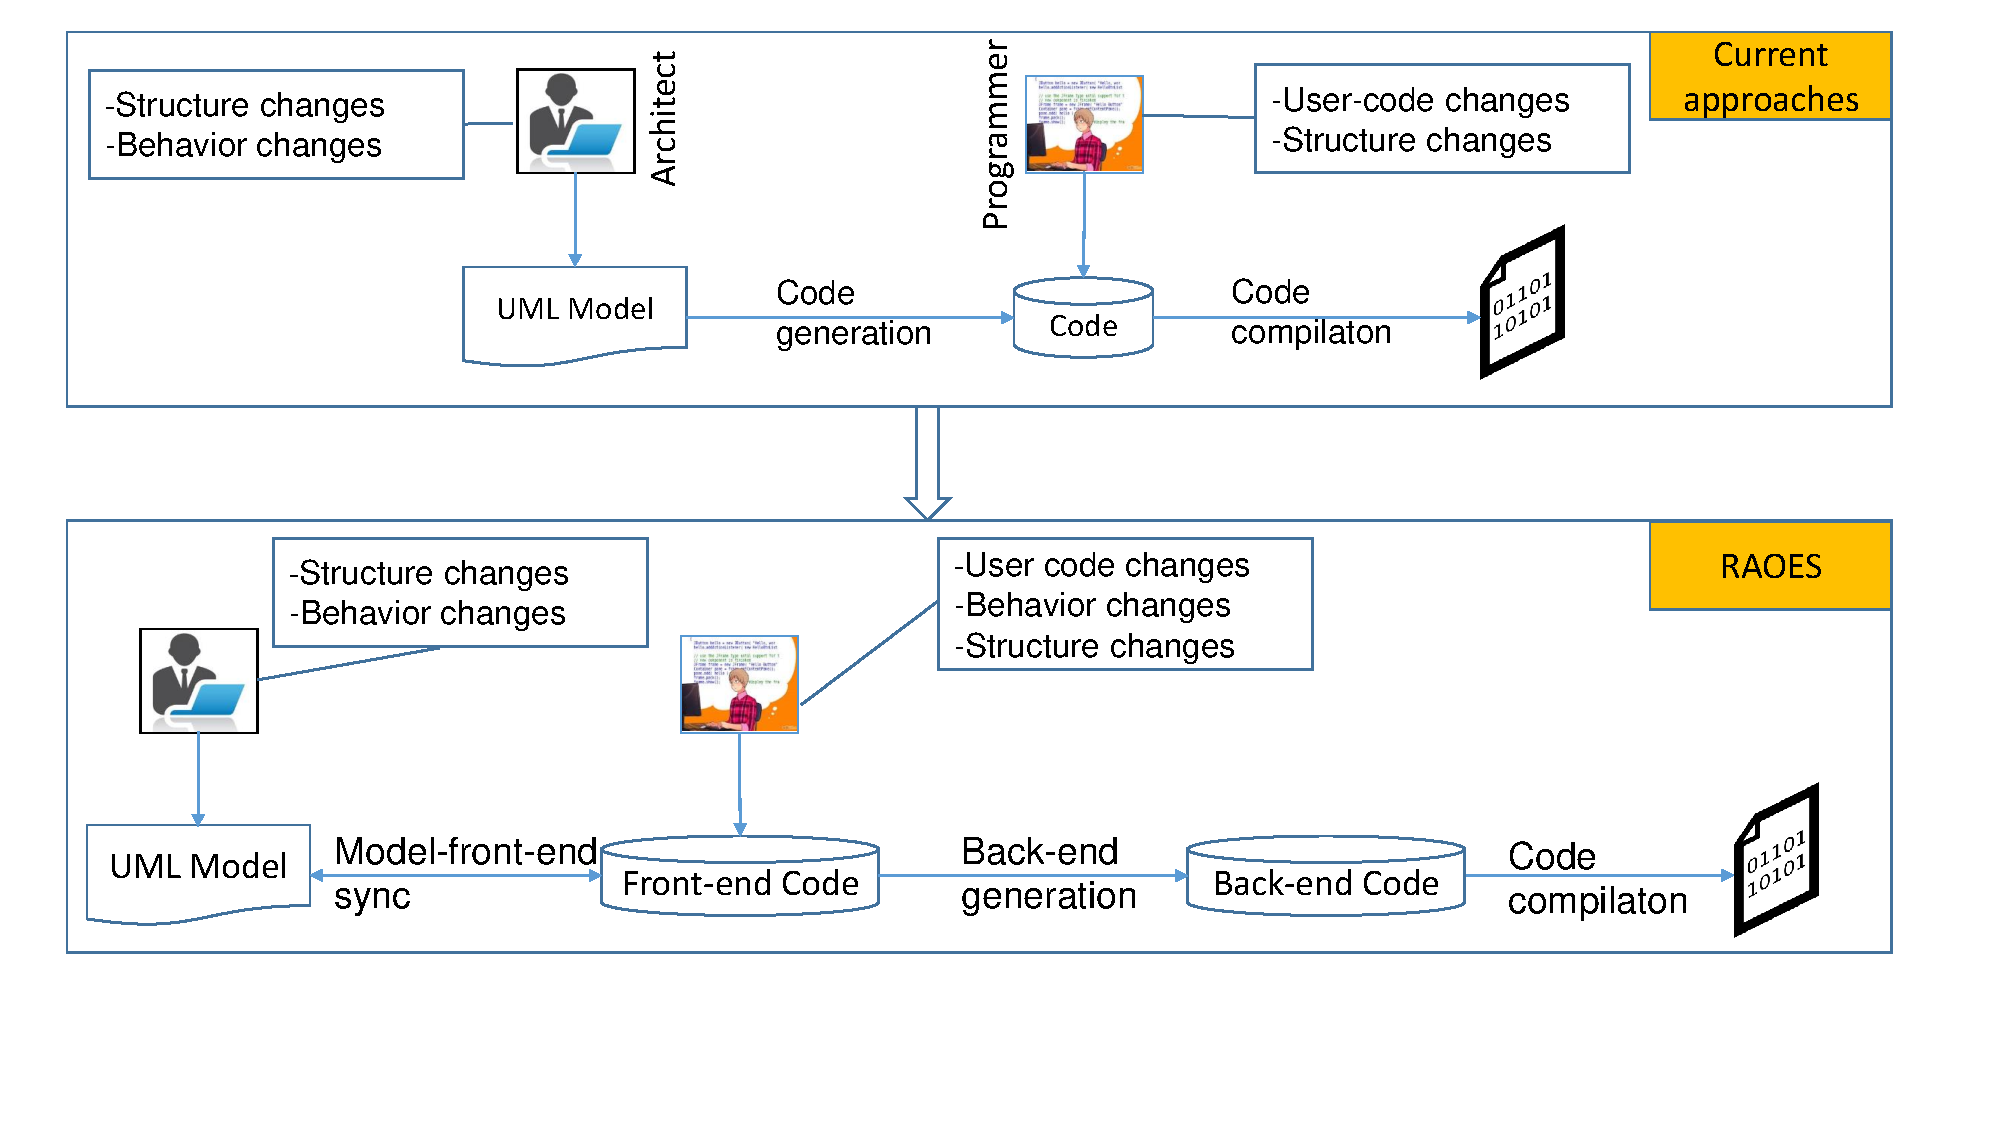
\includegraphics[clip, trim=0.6cm 2.8cm 1.4cm 0.5cm, width=1.0\columnwidth]{figures/frontend}
	\caption{From existing approaches to RAOES} 
	\label{fig:raoes}
\end{figure}

For example, by using RAOES, the generated front-end code for the example in Fig. \ref{fig:IllustrationExample1} and its evolved version are presented in Fig. \ref{fig:frontend-overview}.
The USM defining the behavior of the active class \ti{System} is defined inside the class.
The USM is written in a description-like language.
The topology of the USM is explicitly and hierarchically described.
All USM features can be represented in RAOES's front-end.
Hence, we allow to fully generate code from USMs.

The front-end closely connects to the USM concepts to make programmers easy to modify the state machine.
The front-end merges the USM description into the active class \ti{System} and keeps the class members intact. 
Therefore, the programmers are free to work with C++ as their practice.
This is especially our difference and advantage over some text-based state machine languages such as Umple\footnote{Umple, \url{http://cruise.eecs.uottawa.ca/umple/}} and ThingML\footnote{ThingML, \url{http://thingml.org/}}.
The latter languages adapt existing languages and the programmers' habit into USMs by providing a new language with a new editor (usually defined in Eclipse Xtext).
However, the new editor usually does not support the IDE utilities such as syntax highlights and intelligent completion for mainstream programming languages. 



\begin{figure}
	\centering
	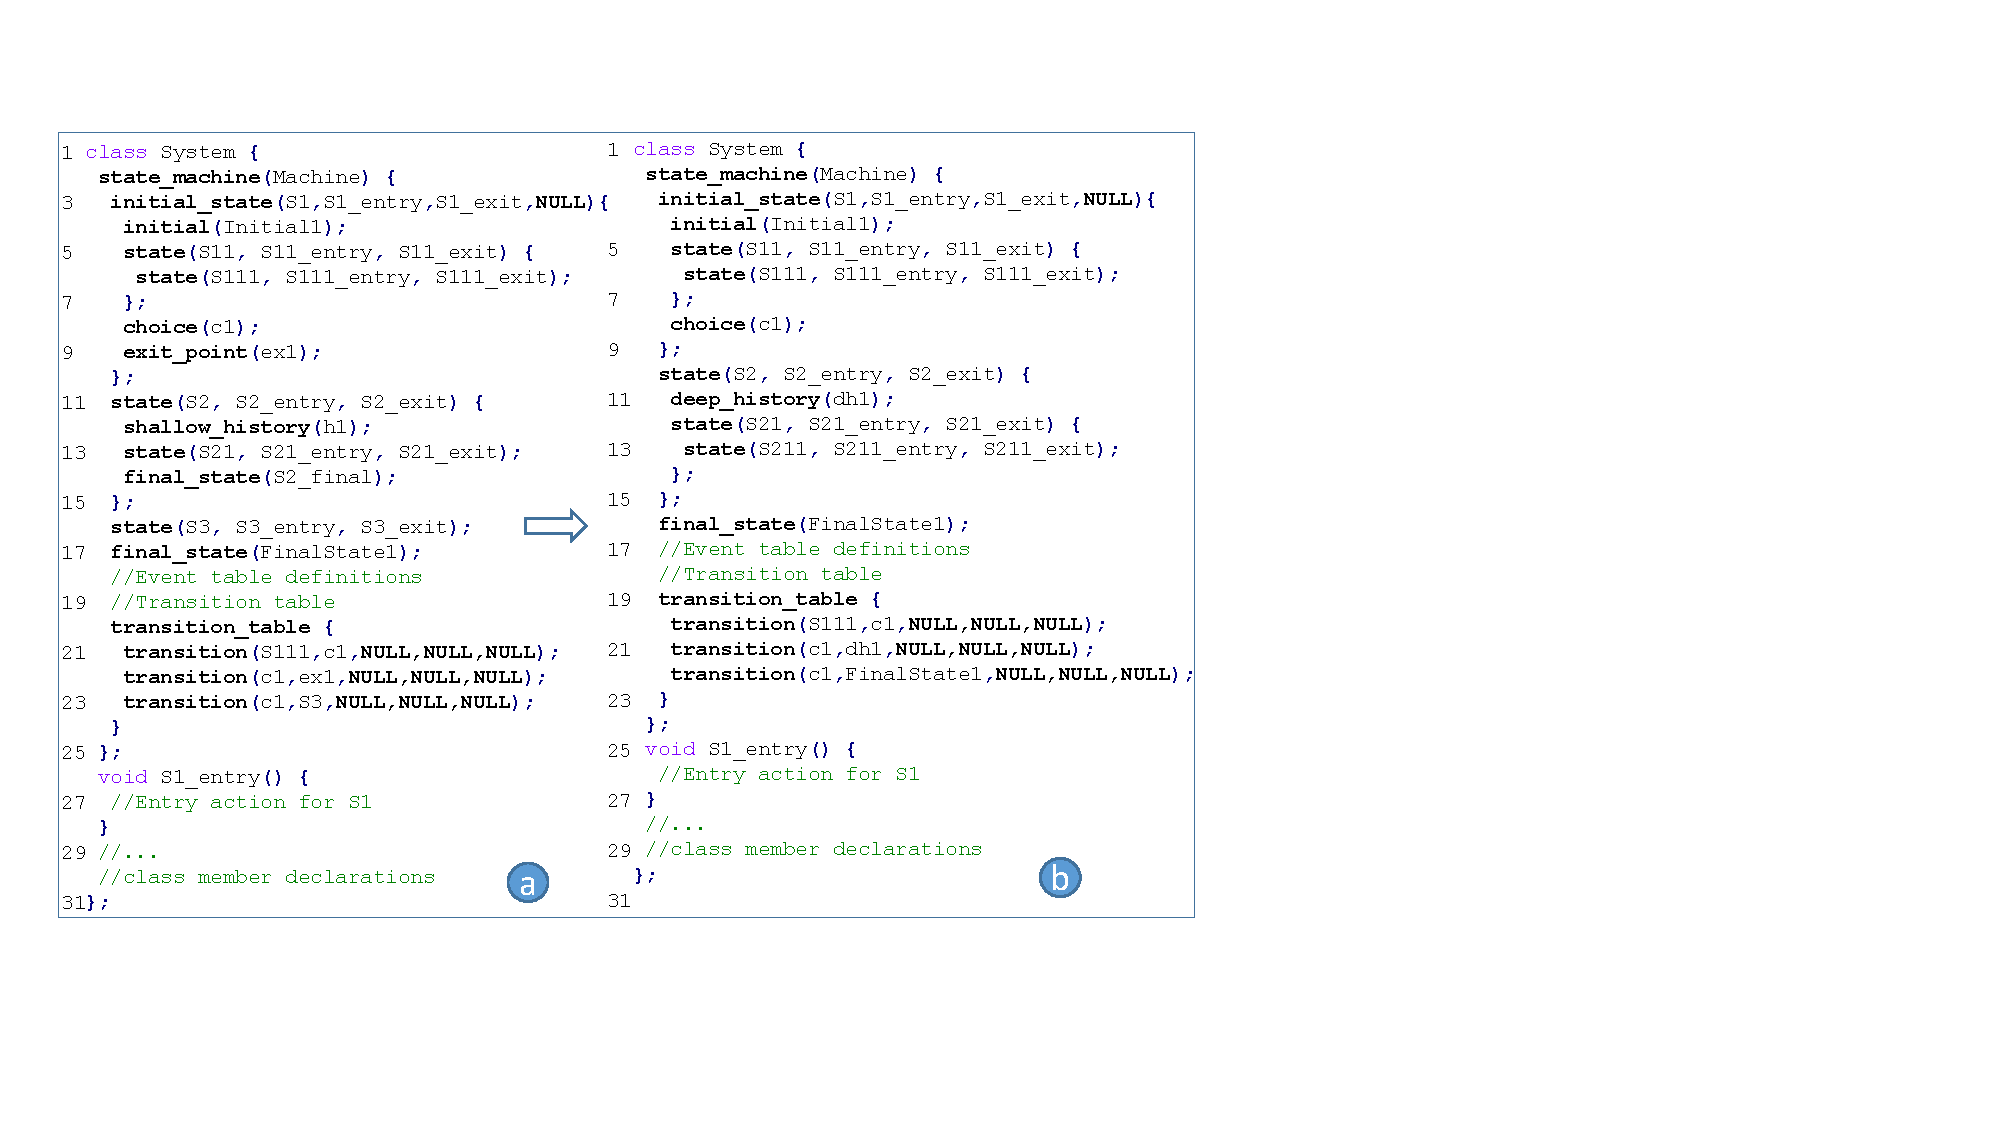
\includegraphics[clip, trim=1.10cm 3.6cm 10.9cm 1.9cm, width=1.08\columnwidth]{figures/frontendoverview.pdf}
	\caption{Front-code evolution} 
	\label{fig:frontend-overview}
\end{figure}